\documentclass[compress]{beamer}
\usefonttheme{professionalfonts}



%

\usepackage[T1]{fontenc}
%\usepackage{kmath,kerkis}
%\usepackage{fouriernc}
\usepackage[adobe-utopia]{mathdesign}
%\usepackage{arev}
\usepackage{times}
\usepackage{natbib}

\usepackage[noend]{algpseudocode}
\usepackage{xmpmulti}
\usepackage{dsfont}
\usepackage{amsmath}

\usepackage{graphicx,float,wrapfig, bbm}
\usepackage{amsfonts, comment, bbold}
\usepackage{mdwlist}
\usepackage{subfigure}
\usepackage{colortbl}
\usepackage{mathrsfs}


\usepackage{multirow}




% packages

\usepackage{amsfonts}

% environments

\newenvironment{packed_enumerate}{
  \begin{enumerate}
    \setlength{\topsep}{0pt}
    \setlength{\itemsep}{2pt}
    \setlength{\parskip}{0pt}
    \setlength{\parsep}{0pt}
}{\end{enumerate}}

\newenvironment{stepit}
 {\begin{itemize}[<+-|alert@+>]}
   {\end{itemize}}

% commands

\newcommand{\Norm}[3]{\mathcal{N}\left( #1, #2, #3 \right)}
\newcommand{\popshow}[2]{\only<#1->{\alert<#1>{#2}}}
\newcommand{\x}{\mathbf{x}}
\newcommand{\ex}[1]{\mbox{exp}\left\{ #1\right\} }
\newcommand{\e}[2]{\mathbb{E}_{#1}\left[ #2 \right] }
\newcommand{\g}{\, | \,}
\newcommand{\indpt}{\protect\mathpalette{\protect\independenT}{\perp}}
\def\independenT#1#2{\mathrel{\rlap{$#1#2$}\mkern2mu{#1#2}}}
\newcommand{\E}{\textrm{E}}
\newcommand{\R}{\textrm{R}}
\newcommand{\realline}{\mathbb{R}}
\newcommand{\data}{{\cal D}}
\newcommand{\loglik}{{\cal L}}
\newcommand{\grad}[2]{ \frac{\partial{#1}}{\partial#2}}
\newcommand{\dir}[1]{\mbox{Dir}(#1)}
\newcommand{\mult}[1]{\mbox{Mult}( #1)}
\newcommand{\G}[1]{\Gamma \left( \textstyle #1 \right)}
\newcommand{\ind}[1]{\mathds{1}\left[ #1 \right] }
\newcommand{\norm}[1]{\left\lVert#1\right\rVert}

\newcommand{\class}[1]{ \texttt{#1}}
\newcommand{\term}[1]{ ``#1''}
\newcommand{\tcword}[0]{ w }
\newcommand{\docsetlabeled}[0]{ D }
\newcommand{\onedoclabeled}[0]{ d }
\newcommand{\tcposindex}[0]{ i }
\newcommand{\myblue}[1]{ {\textbf #1 }}
\newcommand{\dnrm}[1]{ _{\mbox{\textsc{ #1 }}}}
\newcommand{\argmax}[0]{ \arg \max }
\newcommand{\tcjclass}[0]{c_j}
\newcommand{\maths}[1]{ {\bf #1}}




% complexity
\renewcommand{\O}{\mathcal{O}}



\setbeamersize{text margin left=0.5cm}
\setbeamersize{text margin right=0.5cm}
\setbeamercolor{alert}{fg=red!75!black}

\usetheme{default}
\useinnertheme{circles}
\useoutertheme{split}
\usecolortheme{seahorse}
% \usecolortheme{dove}
% \usecolortheme{seagull}
%\usecolortheme{default}
% \usecolortheme{dolphin}
\usefonttheme{structurebold}
%\usefonttheme{serif}

\setbeamertemplate{navigation symbols}{}
\setbeamertemplate{headline}{}
\setbeamertemplate{footline}{}
\setbeamerfont{itemize/enumerate subbody}{size=\normalsize}
\setbeamerfont{itemize/enumerate subsubbody}{size=\normalsize}
\setbeamercolor{itemize item}{fg=gray}
\setbeamercolor{enumerate item}{fg=gray}
\setbeamercolor{itemize item}{fg=gray}
\setbeamercolor{itemize subitem}{fg=gray}
\setbeamercolor{item projected}{bg=gray}
\setbeamercolor{subitem projected}{bg=gray}


\newenvironment{bullets}
{\begin{itemize} \setlength{\itemsep}{10pt}}
{\end{itemize}}

\newcommand{\mygraphic}[2]{
  \begin{beamercolorbox}[colorsep*=4pt]{black math}
    \begin{center}
      \includegraphics[#1]{#2}
    \end{center}
  \end{beamercolorbox}
}

\setbeamercolor{structure}{bg=gray}
\setbeamercolor{section in head/foot}{bg=gray}
\setbeamercolor{palette primary}{bg=lightgray}


\usepackage{minted}

\usetheme[pageofpages=of,                    % String used between the current page and the
                                             % total page count.
          bullet=circle,                     % Use circles instead of squares for bullets.
          titleline=true,                    % Show a line below the frame title.
          showdate=true,                     % show the date on the title page
          alternativetitlepage=true,         % Use the fancy title page.
          titlepagelogo=../../common/culogo,              % Logo for the first page.
          % Logo for the header on first page.
          headerlogo=../../common/boulder_cs,
          ]{UCBoulder}

\usecolortheme{ucdblack}
\author{Introduction to Data Science Algorithms}


\institute[Boyd-Graber and Paul] % (optional, but mostly needed)
{Jordan Boyd-Graber and Michael Paul}


\AtBeginSection[] % "Beamer, do the following at the start of every section"
{ \begin{frame} \frametitle{Outline} % make a frame titled "Outline"
\tableofcontents[currentsection] % show TOC and highlight current section
\end{frame} }


\newcommand{\gfx}[2]{
\begin{center}
	\includegraphics[width=#2\linewidth]{dpmm/#1}
\end{center}
}
\title{Bayesian Non-Parametrics}
\date{Slides adapted from Eli Bingham and Matt Dickenson}

\begin{document}


%%%%%%%%%%%%%%%%%%%%%%%%%%%%%%%%%%%%%%%%%
\begin{frame}
\titlepage
\end{frame}
%%%%%%%%%%%%%%%%%%%%%%%%%%%%%%%%%%%%%%%%%
\begin{frame}
\frametitle{Outline}
\begin{enumerate}
\item Latent feature models
\item Finite latent {\bf feature} (i.e. binary) models
\item (Very fast introduction)
\item Application: Topic Models
\end{enumerate}
\end{frame}
%%%%%%%%%%%%%%%%%%%%%%%%%%%%%%%%%%%%%%%%%
\begin{frame}
\frametitle{Latent feature models}
\begin{itemize}
\item Feature model: $N$ items described by $K$ features
\item Dense feature model: every feature is present in every item, e.g. PCA
\item Sparse feature model: only some features present in each item, and we can assume feature values and presence are independent:
    \begin{eqnarray*}
        \mathbf{X} &=& \mathbf{A} \otimes \mathbf{Z} \\
        P(\mathbf{X}) &=& P(\mathbf{A})P(\mathbf{Z})
    \end{eqnarray*}
\end{itemize}

\begin{figure}
\begin{center}
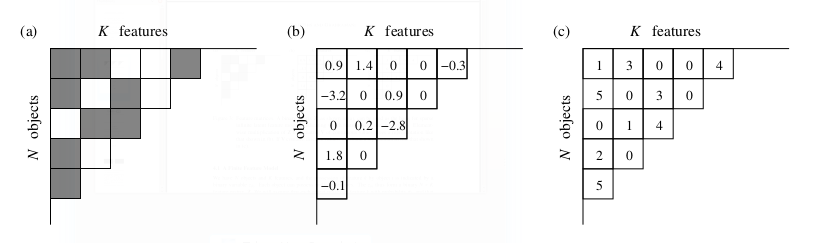
\includegraphics[scale=0.4]{ibp/featuremodel.png}
\caption{Griffiths and Ghahramani (2011) Figure 3}
\end{center}
\end{figure}
\end{frame}
%%%%%%%%%%%%%%%%%%%%%%%%%%%%%%%%%%%%%%%%%
\begin{frame}
\frametitle{Example}

\begin{figure}
\begin{center}
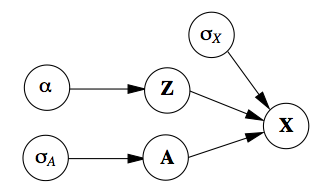
\includegraphics[scale=0.3]{ibp/graphical-model-gaussian.png}
\caption{Griffiths and Ghahramani (2011) Figure 7}
\end{center}
\end{figure}

\begin{figure}
\begin{center}
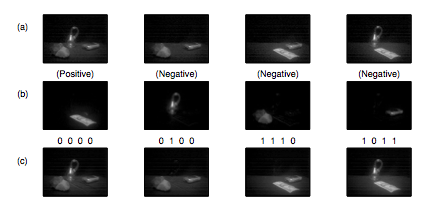
\includegraphics[scale=0.5]{ibp/ibp-example-photos.png}
\caption{Griffiths and Ghahramani (2011) Figure 9}
\end{center}
\end{figure}

\end{frame}
%%%%%%%%%%%%%%%%%%%%%%%%%%%%%%%%%%%%%%%%%
\begin{frame}
\frametitle{Motivation}
\begin{itemize}
\item Problem with finite latent feature model: $K$ is fixed
\item Goal: construct nonparametric prior on $\mathbf{Z}$ so that $K$ grows with the complexity of the dataset
\item As with DPMMs, we can try to build one by taking $K \rightarrow \infty$ in a finite feature model
\end{itemize}

\begin{figure}
\begin{center}
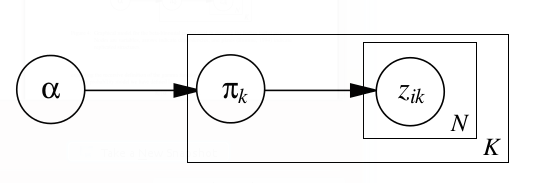
\includegraphics[scale=0.4]{ibp/beta-bernoulli.png}
\caption{Griffiths and Ghahramani (2011) Figure 4}
\end{center}
\end{figure}
\end{frame}
%%%%%%%%%%%%%%%%%%%%%%%%%%%%%%%%%%%%%%%%%


%%%%%%%%%%%%%%%%%%%%%%%%%%%%%%%%%%%%%%%%%
\begin{frame}
\frametitle{Finite latent feature models}
The basic finite distribution on $z_{i,k}$s:
\begin{eqnarray*}
    \pi_k | \alpha &\sim& \text{Beta} \left(\frac{\alpha}{K}, 1 \right) \\
    z_{i,k} | \pi_k &\sim& \text{Bernoulli}(\pi_k)
\end{eqnarray*}
As with DPMMs, we can marginalize out latent feature presence probabilities $\pi_k$ to obtain a distribution on matrices $\mathbf{Z} \in \left\{ 0,1 \right\}^{N \times K}$:
\begin{eqnarray*}
    P(\mathbf{Z}) &=& \prod_{k=1}^K \int \left( \prod_{i=1}^N P(z_{ik} | \pi_k) \right) P(\pi_k) d \pi_k \\
    &=& \prod_{k=1}^K \frac{ \frac{\alpha}{K} \Gamma(m_k + \frac{\alpha}{K} ) \Gamma(N - m_k + 1) }{\Gamma(N + 1 + \frac{\alpha}{K}) }
\end{eqnarray*}
\end{frame}
%%%%%%%%%%%%%%%%%%%%%%%%%%%%%%%%%%%%%%%%%
\begin{frame}
\frametitle{The $K \rightarrow \infty$ limit}
\begin{itemize}
\item $\mbox{lof}(\mathbf{Z})$ is the matrix obtained by ordering the columns of $\mathbf{Z}$ as $N$-digit binary numbers
\item To define a probability over infinitely wide binary matrices using de Finetti's Theorem,
we need exchangeable symmetry, so we define \emph{lof} equivalence classes by modding out column order:
\end{itemize}

\begin{figure}
\begin{center}
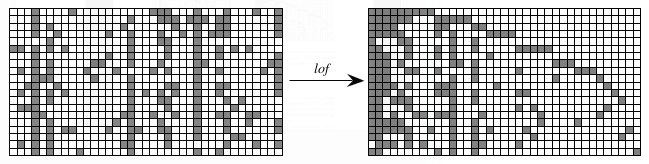
\includegraphics[scale=0.5]{ibp/ibp-sorted.png}
\caption{Griffiths and Ghahramani (2011) Figure 5}
\end{center}
\end{figure}
\end{frame}
%%%%%%%%%%%%%%%%%%%%%%%%%%%%%%%%%%%%%%%%%
\begin{frame}
\frametitle{Indian Buffet Process}

Indian Buffet Process:
\begin{enumerate}
\item $N$ customers enter (in sequence) a buffet restaurant with an infinite number of dishes
\item First customer fills her plate with Poisson($\alpha$) number of dishes
\item $i^{th}$ customer samples dishes in proportion to their popularity, with probability $\frac{m_k}{i}$, where $m_k$ is the number of previous customers who sampled dish $k$
\item $i^{th}$ customer then samples $K^{(i)}_1 \sim \text{Poisson}(\frac{\alpha}{i})$ number of new dishes
\end{enumerate}
\bigskip
Resulting probability distribution on matrices: $$P(\mathbf{Z}) = \frac{\alpha^{K_+}}{\prod_{i=1}^N K^{(i)}_1 ! } \text{exp}(\alpha H_N) \prod_{k=1}^{K_+} \frac{(N - m_k)! (m_k - 1)!}{N!} $$
\end{frame}
%%%%%%%%%%%%%%%%%%%%%%%%%%%%%%%%%%%%%%%%%
\begin{frame}
\frametitle{Alternative derivation: Stick-Breaking}

\begin{enumerate}
\item Recursively break (an initially unit-length) stick, breaking off a $\text{Beta}(\alpha, 1)$ portion at each step
\item Let each portion of the ``stick'', $\pi_k$ represent the probability of each feature (sorted from largest to smallest)
\end{enumerate}

This helps to show the relation between the Dirichlet process and the IBP. The stick-breaking construction is also useful for defining inference algorithms.

\end{frame}
%%%%%%%%%%%%%%%%%%%%%%%%%%%%%%%%%%%%%%%%%
\begin{frame}
\frametitle{Application: Topic Modeling}
% Williamson, Wang, Heller, and Blei (2010)

\begin{center}
``The IBP Compound Dirichlet Process \\
and its Application to Focused Topic Modeling'' \\
Williamson, Wang, Heller, and Blei (2010)
\end{center}

Stick-breaking construction:

\begin{eqnarray*}
\mu_k \sim \text{Beta}(\alpha, 1) \\
\pi_k = \prod_{j=1}^k \mu_j \\
b_{m,k} \sim \text{Bernoulli}(\pi_k)
\end{eqnarray*}


\end{frame}
%%%%%%%%%%%%%%%%%%%%%%%%%%%%%%%%%%%%%%%%%
\begin{frame}
\frametitle{Application: Topic Modeling}
% Williamson, Wang, Heller, and Blei (2010)

% \begin{center}
% ``The IBP Compound Dirichlet Process \\
% and its Application to Focused Topic Modeling'' \\
% Williamson, Wang, Heller, and Blei (2010)
% \end{center}

Focused topic model:
\begin{enumerate}
\item for $k=1,2,\ldots$
  \begin{itemize}
  \item Sample stick length $\pi_k$
  \item Sample relative mass $\phi_k \sim \text{Gamma}(\gamma, 1)$
  \item Draw topic distribution over words: $\beta_k \sim \text{Dirichlet}(\eta)$
  \end{itemize}
\item for $m=1,\ldots,M$
  \begin{itemize}
  \item Sample binary vector $b_m$
  \item Draw total number of words $n^{(m)} \sim NB(\sum_k b_{m,k} \phi_k, 1/2)$
  \item Sample distribution over topics $\theta_m \sim \text{Dirichlet}(b_m \cdot \phi)$
  \item For each word $w_{m,i}, i=1,\ldots,n^{(m)}$
    \begin{enumerate}
    \item Draw topic index $z_{m,i} \sim \text{Discrete}(\theta_m)$
    \item Draw word $w_{m,i} \sim \text{Discrete}(\beta_{z_{m_i}})$
    \end{enumerate}
  \end{itemize}
\end{enumerate}

\end{frame}
%%%%%%%%%%%%%%%%%%%%%%%%%%%%%%%%%%%%%%%%%
\begin{frame}
\frametitle{Application: Topic Modeling}
% Williamson, Wang, Heller, and Blei (2010)



% \begin{center}
% ``The IBP Compound Dirichlet Process \\
% and its Application to Focused Topic Modeling'' \\
% Williamson, Wang, Heller, and Blei (2010)
% \end{center}

\begin{columns}
  \column{.5\linewidth}
  \begin{center}
  Number of Topics a Word Appears in
  \end{center}
  \column{.5\linewidth}
  \begin{center}
  Number of Documents a Topic Appears in
  \end{center}
\end{columns}

\gfx{focused-tm}{.8}

\begin{itemize}
  \item Separates global topic proportions from per-document
    distribution
  \item Rare topics can dominate documents
  \item Frequent topics can't appear in as many documents
\end{itemize}

\end{frame}
%%%%%%%%%%%%%%%%%%%%%%%%%%%%%%%%%%%%%%%%
\begin{frame}
\frametitle{Discussion}


Limitations of IBP:
\begin{enumerate}
\item Coupling of average number of features $\alpha$ and total number of features $N\alpha$ (can be overcome with a two-parameter generalization)
\item Computationally complex, can be time-consuming
\end{enumerate}

\begin{figure}
\begin{center}
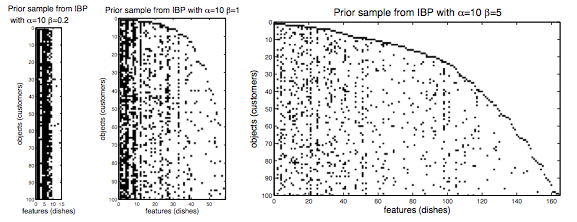
\includegraphics[scale=0.3]{ibp/two-parameter-ibp.png}
\caption{Griffiths and Ghahramani (2011) Figure 10}
\end{center}
\end{figure}

\end{frame}


\begin{frame}{Connection to Rest of Course}

  \begin{itemize}
    \item[+] Bayesian Nonparameterics discovers dimension
    \item[+] Strong probabilistic foundations
    \item[+] Gives meaning to representation
    \item[-] Hard to implement
    \item[-] Slow
    \item[-] Not as effective
  \end{itemize}

\end{frame}

% End of slides
\end{document}
